\documentclass[journal]{vgtc} 
\usepackage{hs-vis_ws1819}
\usepackage{url}


%% Please note that the use of figures other than the optional teaser
%% is not permitted on the first page of the journal version.  Figures
%% should begin on the second page and be in CMYK or Grey scale
%% format, otherwise, colour shifting may occur during the printing
%% process.  Papers submitted with figures other than the optional
%% teaser on the first page will be refused.

%% These three lines bring in essential packages: ``mathptmx'' for
%% Type 1 typefaces, ``graphicx'' for inclusion of EPS figures. and
%% ``times'' for proper handling of the times font family.

\usepackage{mathptmx} 
\usepackage{graphicx}
\usepackage{times}
\usepackage[space]{grffile}
\usepackage{hyperref}


%% allow for this line if you want the electronic option to work
%% properly
\vgtcinsertpkg


%% author name
\author{Dominik Sellenthin \and Michael Stegmaier \and Gariharan Kanthasamy}

%% paper title
\title{OpenGL-basiertes Software Occlusion Culling zur Beschleunigung des 3D-Renderings gro{\ss}er Datenmengen und komplexer Szenen}

%% short title for header
\shorttitle{Software Occlusion Culling}


%% Abstract section.
\abstract{%

%%% ÜBERARBEITUNG BENÖTIGT %%%
In Bereichen des 3D-Rendering, sei es in der wissenschaftlichen Visualisierung oder in Computerspielen, ist die Rechenleistung der Grafikkarte schnell an ihrer Grenze, w"ahrend die CPU kaum in Anspruch genommen wird. Damit die GPU entlastet wird, wird ein Software-Rasterisierer eingesetzt, so dass ein Teil der Berechnungen in einem Vorverarbeitungsschritt auf die CPU ausgelagert wird. Um die vollst"andige Rechenleistung moderner Multi-Core CPUs zu gew"ahrleisten, wird in dieser Arbeit ein bereits vorhandener Rasterierer, Mesa 3D, verwendet, der zus"atzlich die OpenGL API zur Verf"ugung stellt. Ziel des Software-Rasterisierers ist es, komplett parallel zum GPU-Rendering des aktuellen Frames, in zwei Schritten festzustellen, welche Objekte in der kommenden Szene zu sehen sind. Im Wesentlichen gilt es dabei zuerst einen geeigneten Tiefenpuffer zu generieren und anschlie{\ss}end mittels Occlusion Queries alle Objekte zu bestimmen, die noch sichtbar sind (auch Z-Buffering genannt). Das Ergebnis der Occlusion Queries kann nun ohne nennenswerte Latenz verwendet werden, um der GPU mitzuteilen, welche Objekte gerendert werden sollen, so dass unn"otiger Rechenaufwand der GPU vermieden wird (~160).
} % end of abstract


%% Uncomment below to include a (optional) teaser figure.
\teaser{ \centering
  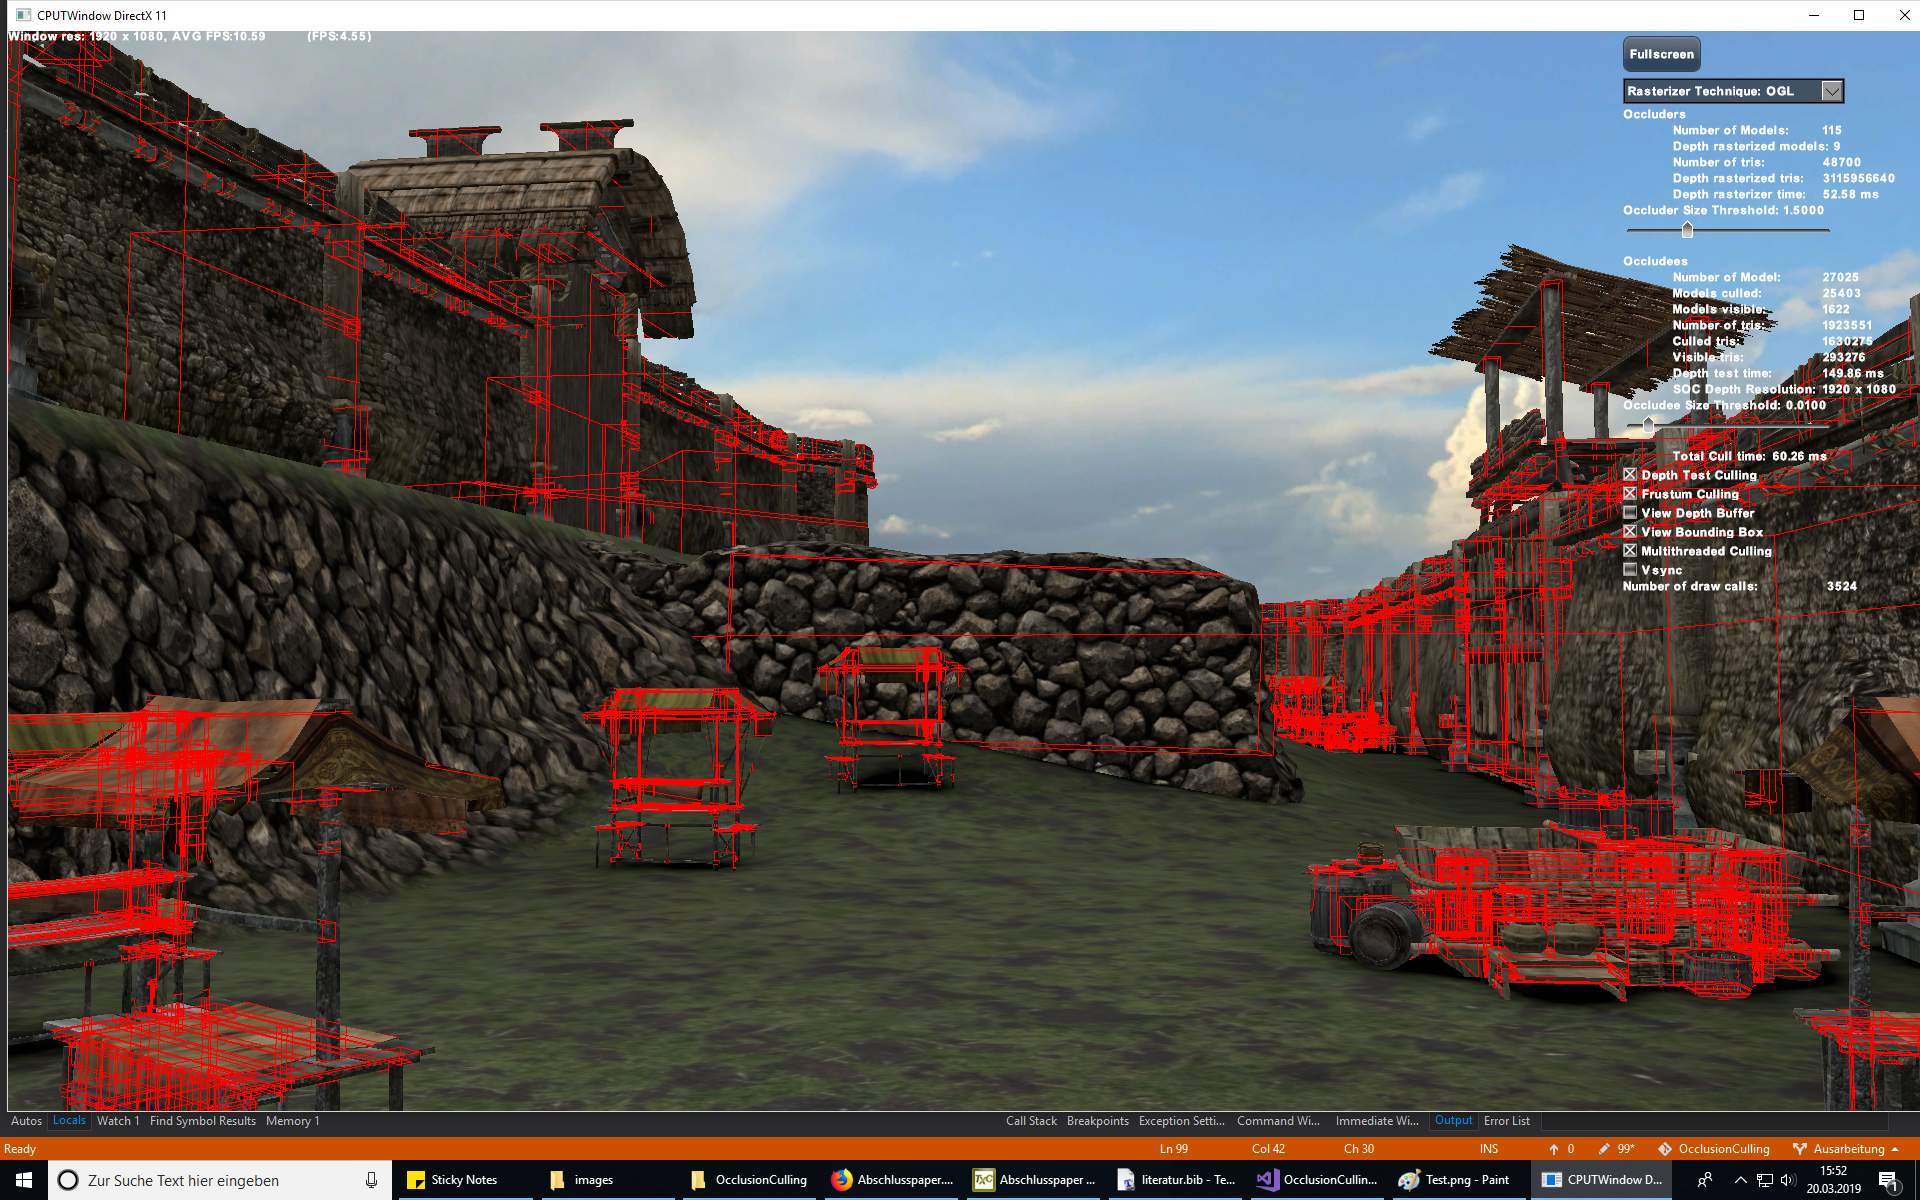
\includegraphics[width=\columnwidth]{images/Base1AABB.png}%
	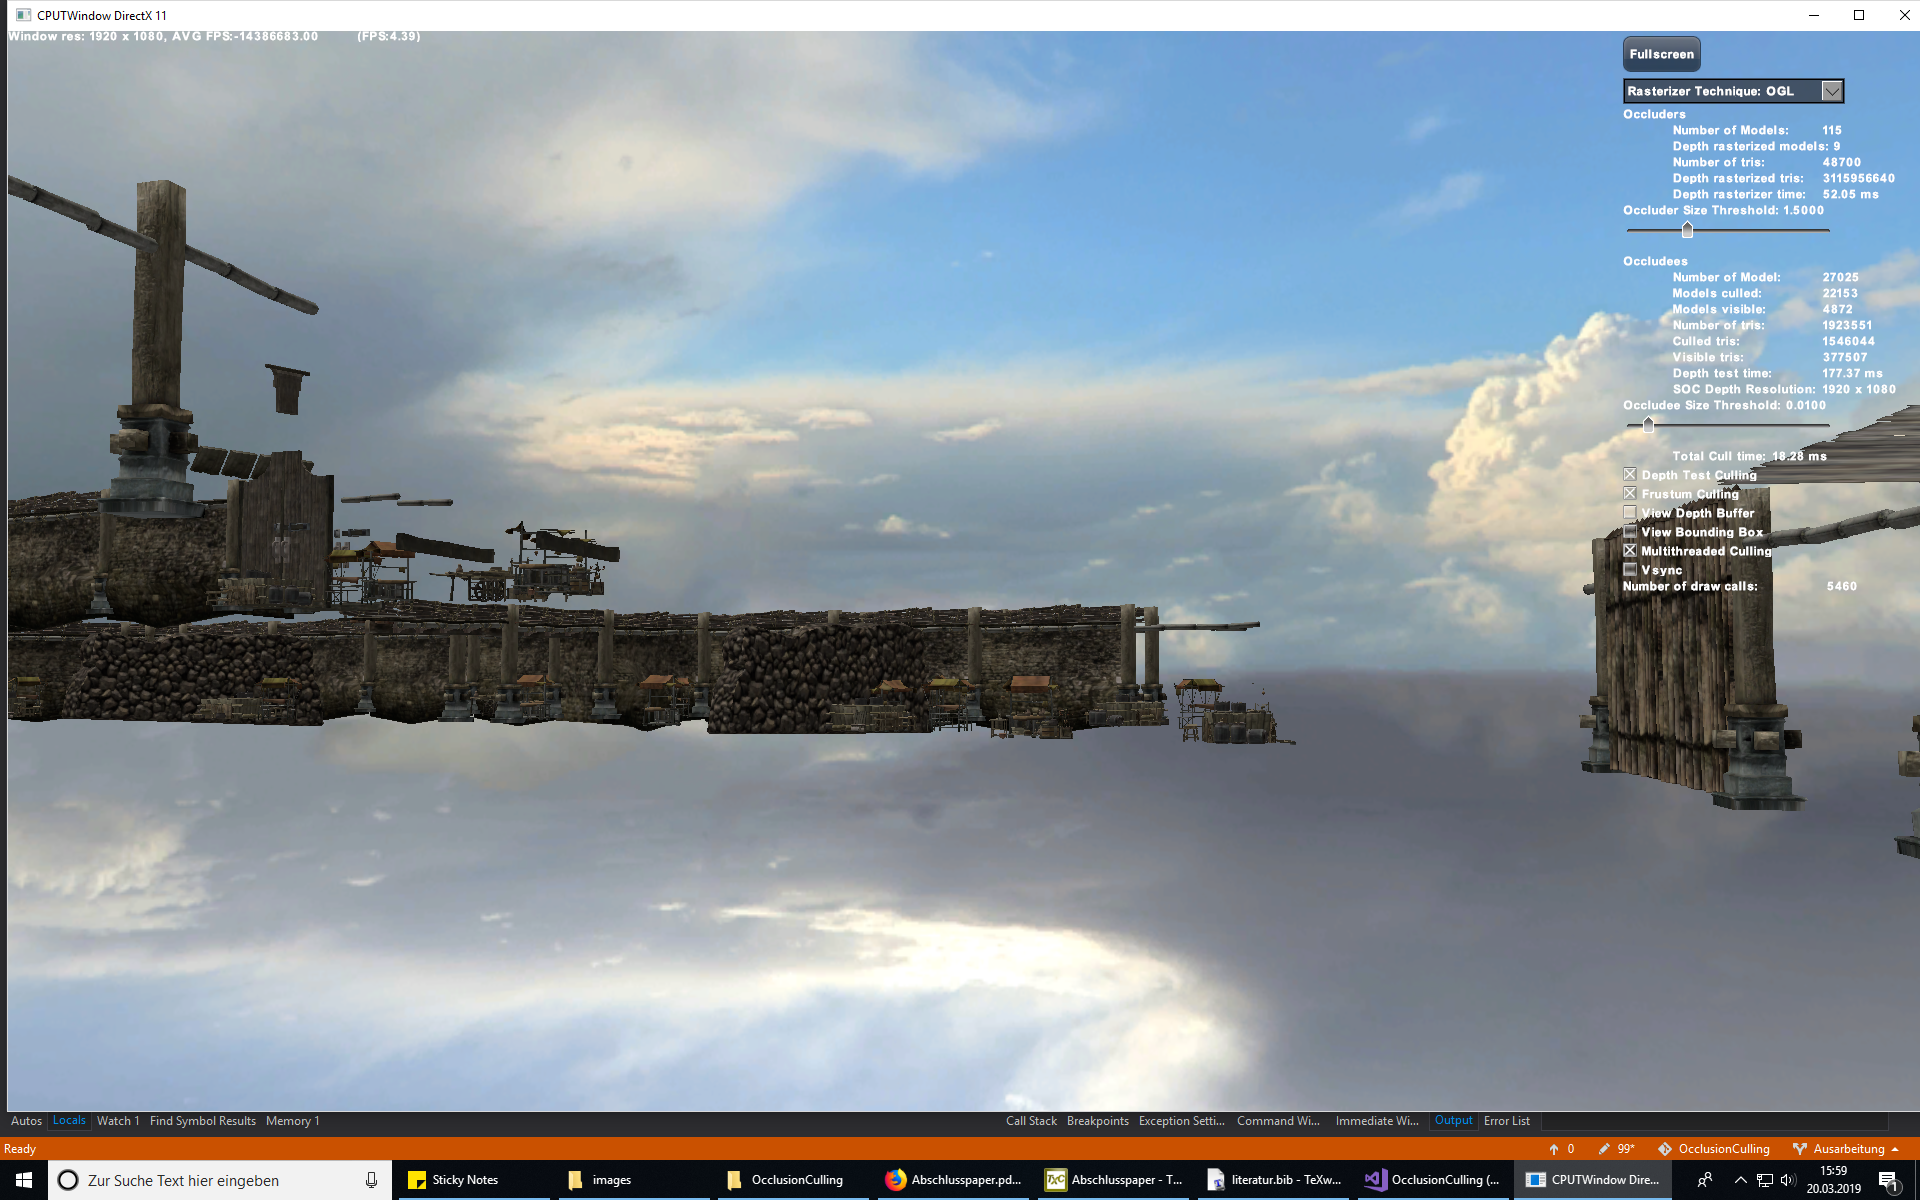
\includegraphics[width=\columnwidth]{images/Base1Invert.png}%
	\caption{Links: Testergebnisbild nach einem erfolgreichen Durchlauf der OGL-Methode aus der verwendeten Intel-Testszene. Rote Linien um Objekte stellen die Axis Aligned Bounding Box des jeweiligen Objekts dar. Rechts: Bild aller Objekte, die beim Occlusion Culling als verdeckt klassifiziert wurden und im linken Bild nicht gerendert wurden.}%
	\label{fig:teaser}
}


%%%%%%%%%%%%%%%%%%%%%%%%%%%%%%%%%%%%%%%%%%%%%%%%%%%%%%%%%%%%%%%%
%%%%%%%%%%%%%%%%%%%%%% START OF THE PAPER %%%%%%%%%%%%%%%%%%%%%%
%%%%%%%%%%%%%%%%%%%%%%%%%%%%%%%%%%%%%%%%%%%%%%%%%%%%%%%%%%%%%%%%

\begin{document}

%% The ``\maketitle'' command must be the first command after the
%% ``\begin{document}'' command. It prepares and prints the title
%%   block.

%%   the only exception to this rule is the \firstsection command
\firstsection{Einleitung}

\maketitle

Egal, ob im Bereich der wissenschaftlichen Visualisierung oder in anderen 3D-Rendering-Bereichen, heutige Anwendungen haben immer h"ohere Anspr"uche an die Leistung der Engines(?) und der Wunsch nach besserer Performanz und h"oheren Bildraten (frames per second, FPS) ist gro{\ss}. Hinzukommt, dass in modernen Anwendungen die zu rendernden Szenen immer weniger statisch und immer mehr dynamisch werden, wie es beispielsweise in Computerspielen der Fall ist. Um dieser Dynamik gerecht zu werden, wird sich von Verfahren mit potenziellen Sichtbarkeitsmengen entfernt\cite{MSOC} und es wird sich einer Methode namens \textit{Occlusion Culling} (\textit{to occlude = verdecken, to cull = aussondern, herausfiltern}) bedient. Ziel des Occlusion Cullings ist es, noch vor dem Rendering der n"achsten Szene, herauszufinden, welche Objekte in der kommenden Szene sichtbar sind und welche nicht. Im Wesentlichen gilt es dabei zuerst mit einer ausgew"ahlten Teilmenge der Objekte einen geeigneten Tiefenpuffer (Z-Buffer) zu generieren und darauffolgend mit Hilfe von Occlusion Queries alle Objekte zu bestimmen, die noch sichtbar sind (auch Z-Buffering oder Tiefentest genannt). Das Ergebnis der Occlusion Queries kann anschlie{\ss}end ohne nennenswerte Latenz verwendet werden, um der GPU mitzuteilen, welche Objekte gerendert werden sollen, so dass unn"otiger Rechenaufwand der GPU vermieden wird.

Bei Anwendungen, die ohnehin schon enormen Rechenaufwand ben"otigen und die maximale Rechenkapazit"at der Grafikkarte schnell ausreizen, ist es schwierig den zus"atzlichen Mehraufwand ebenfalls der Grafikkarte aufzuerlegen. Es bietet sich daher an, den Mehraufwand dem wenig genutzten Prozessor zu "ubergeben, der dann komplett parallel zur Grafikkarte das Occlusion Culling in einem Vorverarbeitungsschritt durchf"uhren soll, siehe Abb.\ \ref{fig:ablauf}.

\begin{figure}%
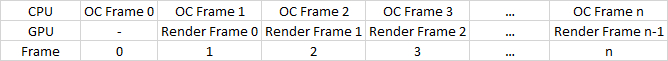
\includegraphics[width=\columnwidth]{images/Ablauf.PNG}%
\caption{Prozessor berechnet parallel zum Rendering der Grafikkarte, welche Objekte in der n"achsten Szene zu sehen sind.}%
\label{fig:ablauf}%
\end{figure}

Moderne Prozessoren besitzen mittlerweile einige separat nutzbare Kerne, die parallel verwendet werden k"onnen, um das Occlusion Culling so effektiv und effizient wie m"oglich zu implementieren. Damit die gesamte Rechenleistung der Prozessoren auch genutzt wird, wird in dieser Arbeit auf den Software-Rasterisierer Mesa 3D zur"uckgegriffen, der au{\ss}erdem mit der bew"ahrten OpenGL API arbeitet. 

Implementiert wurde die OGL-Methode in einem Software Occlusion Culling (SOC) Framework, das von Intel frei zur Verf"ugung gestellt wird \cite{SOCF}. Das Framework eignet sich sehr gut f"ur die Implementierung einer neuen SOC-Methode, da es sowohl essentielle Ablaufstrukturen als auch eine ausreichend gro{\ss}e und komplexe Testszene zur Verf"ugung stellt, mit der eine Evaluation der OGL-Methode erm"oglicht wird, siehe Abb.\ \ref{fig:teaser} links.


\section{Related Work}
Diese Arbeit orientiert sich stark an Intels SOC-Framework, in das die in dieser Arbeit entwickelte OGL-Methode eingebettet wurde. Da das Framework bereits alle notwendigen Strukturen f"ur schon bestehende Methoden besitzt (siehe Abb.\ \ref{fig:ablaufframework}), gestaltet sich die Erweiterung um eine weitere Methode gr"o{\ss}tenteils unkompliziert. 
\begin{figure}%
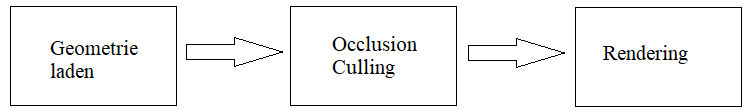
\includegraphics[width=\columnwidth]{images/AblaufFramework.png}%
\caption{Verwende gr"o{\ss}tenteils vorhandene Strukturen, um die verwendete Geometrie zu laden. Anschlie{\ss}end erfolgt das Culling durch die neue OGL-Culling-Methode. Zum Schluss wird die nicht gecullte Geometrie an das Framework zur"uckgegeben, damit das Ergebnis gerendert wird.}%
\label{fig:ablaufframework}%
\end{figure}
Hinzukommen lediglich Ver"anderungen der Routinen zum Laden der Testszene und die Implementierung des Cullings selber. Vorhanden sind unter anderem Methoden, die mit \textit{Streaming SIMD Extension} (SSE) und \textit{Intel Advanced Vector Extension} (AVX) arbeiten. Au{\ss}erdem ist noch eine optimierte Variante der AVX-Technik vorhanden, \textit{Masked Software Occlusion Culling} (MSOC) \cite{MSOC}, die mit einer abgewandelten Form des hierarchischen Z-Buffers (HiZ) \cite{HiZ} arbeitet, der durch einen Software-Rasterisierer berechnet wird.

Hasselgren et al. \cite{MSOC} stellen in ihrer Arbeit einen Algorithmus vor, der durch seinen effizienten HiZ die Performanz signifikant verbessert. Anstatt wie in fr"uheren Arbeiten Pixel als kleinste Einheit zu betrachten, werden nun \textit{Kacheln} verwendet. Kacheln sind dabei lediglich eine Zusammenfassung mehrerer aneinanderliegender Pixel. Da AVX2 erm"oglicht, 8 SIMD Instruktionen mit 32-Bit Pr"azision auszuf"uhren, wurde f"ur die Kacheln eine Gr"o\ss{}e von 32x8 Pixeln gew"ahlt. Indem Bitmasken von rechts und links in die Kacheln geschoben werden, wird am Ende eine Abdeckungsmaske erhalten, die angibt, welche Pixel in einer Kachel verdeckt werden \cite{MSOC}.
W"ahrend ihr Algorithmus keine 100\% Pr"azision garantiert - \textit{false positives} sind m"oglich - bewegt sich der Fehler in gleicher Gr"o\ss{}enordnung wie bei bisherigen Algorithmen. Ein wichtiger Faktor f"ur die Performanz ihres Algorithmus ist die Reihenfolge, in der die Objekte gerendert werden. Die Objekte sollten bestm"oglichst von vorne nach hinten gerendert werden. Dadurch werden die wichtigsten Occluder als erstes rasterisiert (dargestellt) und f"ur den Fall, dass die Zeit f"ur Occlusion Culling begrenzt ist, wird trotzdem ein nahezu optimales Ergebnis erzielt \cite{MSOC}.



\section{Software Occlusion Culling}
Die Menge der Objekte, die es zu Rendern gilt, wird in zwei Mengen aufgeteilt. Zum einen gibt es die Occluder. Occluder sind eine Menge von Objekten, die gro{\ss} genug sind, dass es wahrscheinlich ist, dass sie andere Objekte verdecken. Zum anderen gibt es Occludees. Occludees sind all diejenigen Objekte die potentiell von Occludern verdeckt werden (das hei{\ss}t, sie beinhalten ebenfalls alle Occluder). Sowohl Occluder als auch Occludees liegen dabei in zwei Formen vor. Einmal als Netz bestehend aus Punkten (Mesh), das zur exakten Darstellung des Objekts in der gerenderten Szene dient und einmal in Form einer Axis Aligned Bounding Box (AABB), die sowohl zum Frustumculling als auch zum (Tiefen-)Rasterisieren verwendet wird. AABBs eignen sich wegen ihrer einfachen geometrischen Form sehr gut, um erste grobe Tests durchzuf"uhren, ob ein Objekt "uberhaupt von der Kamera gesehen werden kann (Frustumculling) und dementsprechend f"ur die folgende Rasterisierung beim Occlusion Culling in Frage kommt. Ist die AABB au{\ss}erhalb des Sichtfeldes (Frustum) der Kamera, kann das Objekt ebenfalls nicht sichtbar sein und bereits aus der Menge der zu betrachtenden Objekte genommen werden.

Occlusion Culling besteht im Wesentlichen aus zwei Schritten. Als erstes wird der Tiefenpuffer auf Basis einer Occludermenge beschrieben. Diese Occluder werden in einem ersten Renderingdurchlauf rasterisiert, jedoch ohne die Objekte tats"achlich zu zeichnen, und der Tiefenpuffer wird entsprechend der Occludermenge beschrieben, siehe Abb.\ \ref{fig:db}.
\begin{figure}%
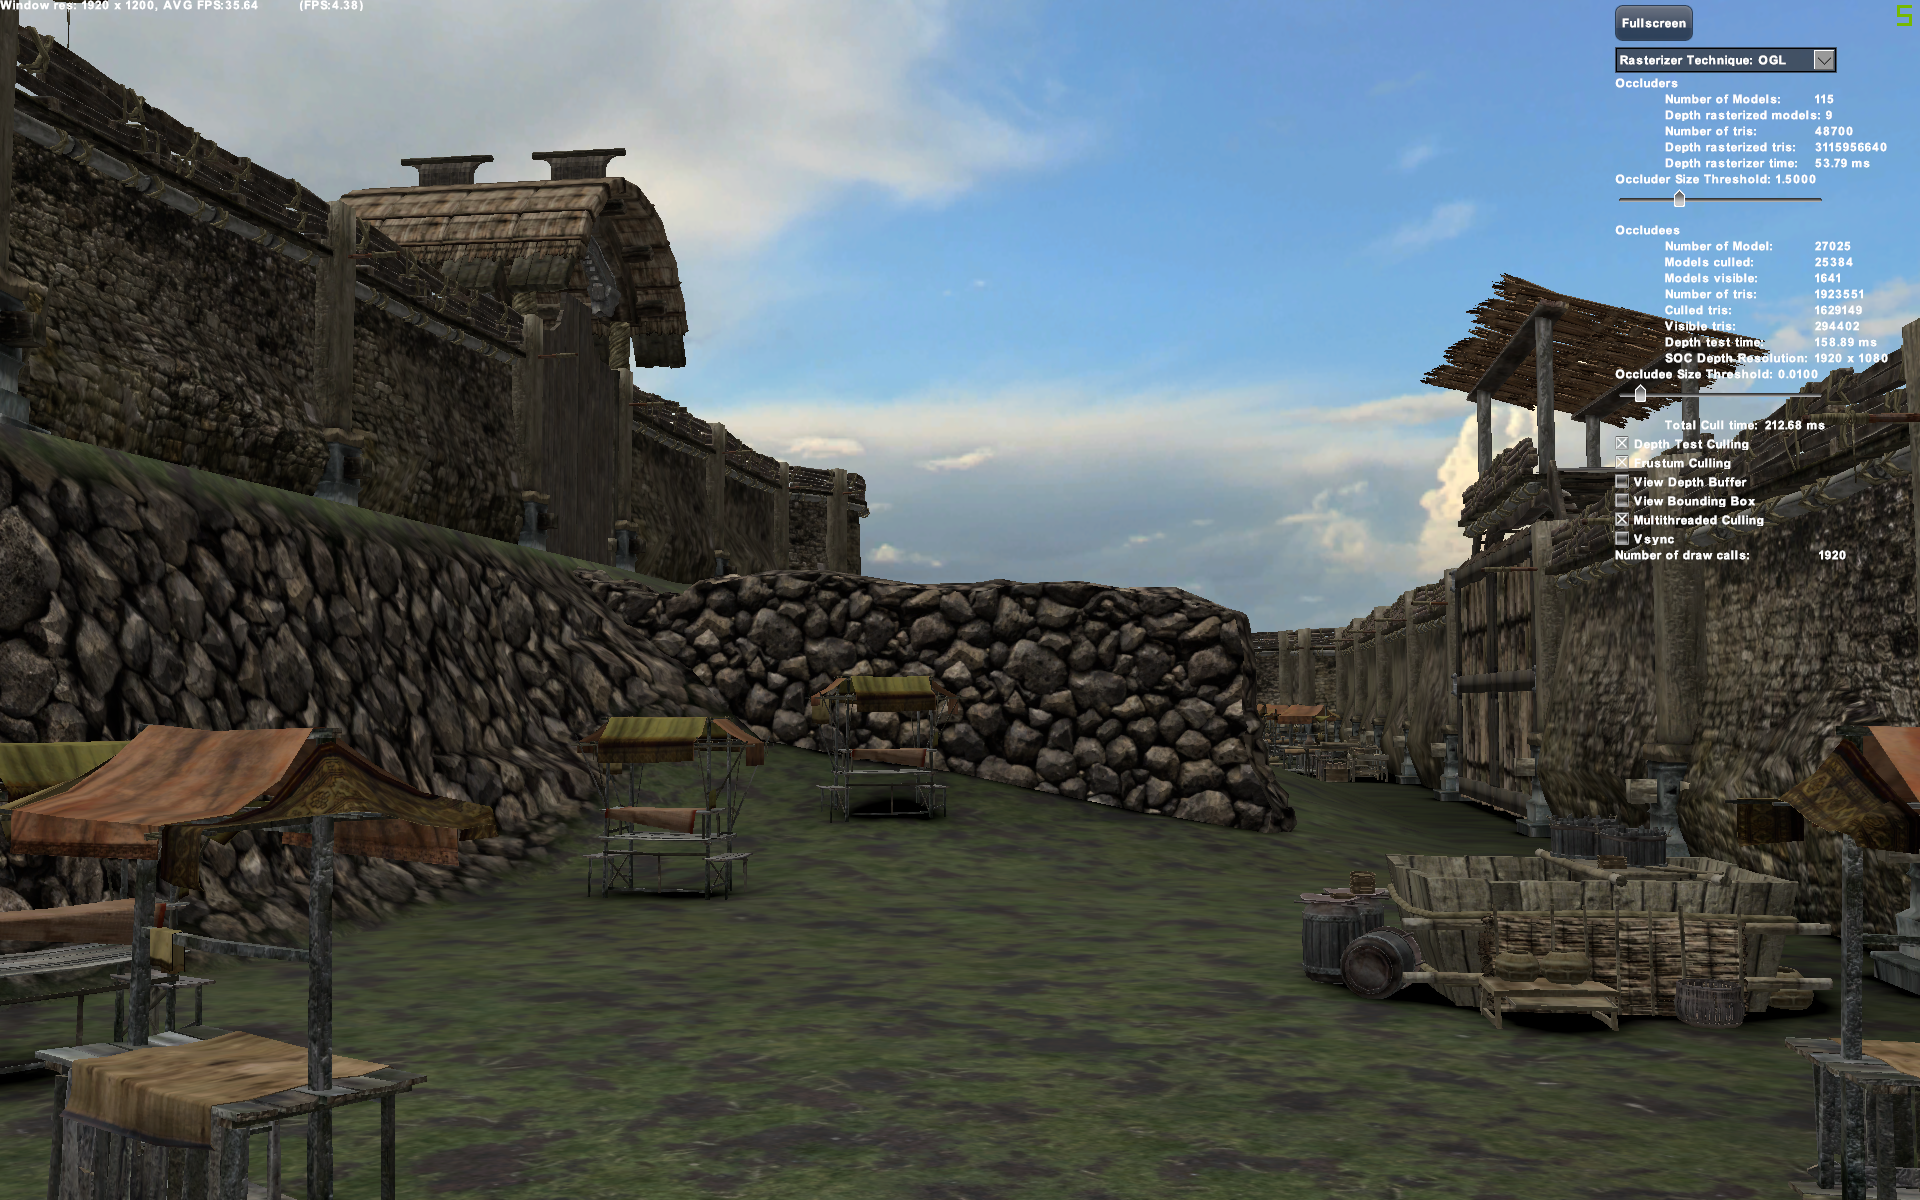
\includegraphics[width=0.5\columnwidth]{images/Base1.png}%
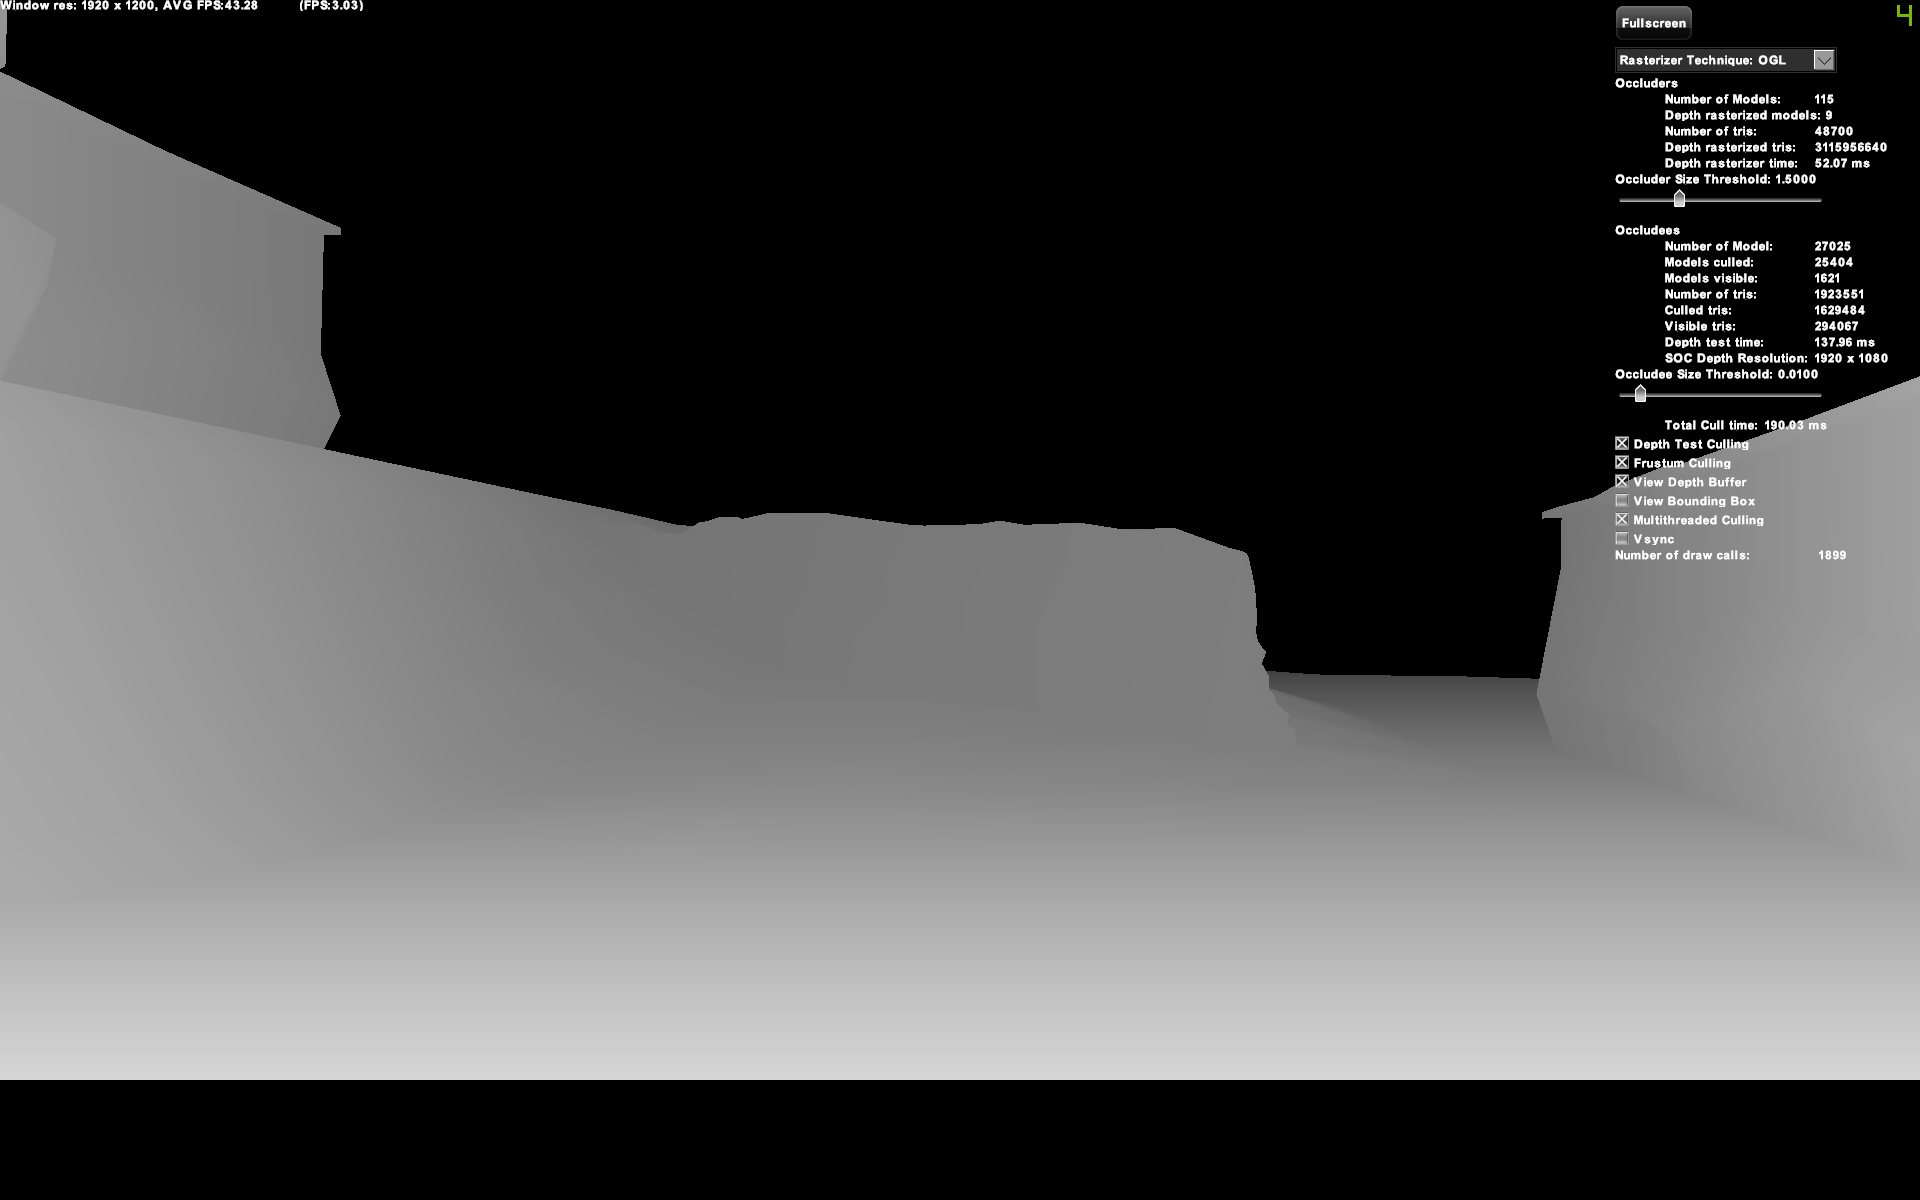
\includegraphics[width=0.5\columnwidth]{images/Base1DB.png}%
\caption{Links: Testbild der Szene. Rechts: Der dazugeh"orige Tiefenpuffer, der in jedem Frame einmal berechnet wird und sp"ater f"ur die Tiefentests der Occlusion Queries verwendet wird.}%
\label{fig:db}%
\end{figure}
Schritt zwei besteht darin Occlusion Queries durchzuf"uhren. Bei den Occlusion Queries werden die Bounding Boxes aller Occludees gegen den im vorherigen Schritt erstellten Tiefenpuffer getestet und es wird gepr"uft, ob die Occludees den Tiefentest bestehen oder nicht, sprich, ob die Occludees von einem Occluder komplett verdeckt werden oder (teilweise) sichtbar sind.\\
Unmittelbar vor jedem dieser beiden Schritte wird zus"atzlich noch Frustumculling durchgef"uhrt, um die Menge der zu testenden Objekte bereits im Vorfeld einzuschr"anken und somit weiter an Performanz zu gewinnen. Der grunds"atzliche Ablauf in jedem Frame sieht also wie folgt aus:\\

\begin{minipage}{0.1\textwidth}\end{minipage}\begin{minipage}{0.4\textwidth}Occluder Frustumculling $\rightarrow$ Tiefenpuffer Rasterisierung\\$\rightarrow$ Occludee Frustumculling $\rightarrow$ Occlusion Queries\\$\rightarrow$ Rendern aller passierten Occludees\end{minipage}


\subsection{Frustumculling}
Frustum Culling rendert nur Objekte die sich im Sichtbereich der Kamera befinden und kann somit je nach Kameraposition einen Teil der Objekte cullen.\\
Vorteil von OC gegen"uber FC (\textbf{ggf bei Ergebnisse}): W"ahrend die Performance des Frustum Cullings sehr konstant bleibt, sind bei den beiden Occlusion Culling Algorithmen gr"o\ss{}ere Schwankungen erkennbar, da ein gro\ss{}er Occluder im Vordergrund potenziell alle Occludees hinter ihm "uberdecken kann und damit die Berechnung stark vereinfacht.\\
\subsection{Tiefenpuffer Rasterisierung}
\subsection{Occlusion Queries}

\section{Ergebnisse}
Daten zur Testszene

Als Basiswert f"ur die Performance des Masked Occlusion Algorithmus (MOC) wurde ein normales Rendering ohne Occlusion Culling, aber mit Frustum Culling verwendet.
Als alternativer Algorithmus wird der \glqq Hierarchical Z Buffer algorithm \grqq{} (HiZ) evaluiert.
Alle Messungen wurden mit voller Aufl"osung (1920*1080 Pixel) ausgef"uhrt, au\ss{}erdem wurde nur die Single-Core Performance betrachtet.
Der MOC Algorithmus ist im Vergleich zum HiZ Algorithmus etwas vorsichtiger und cullt 2\% weniger Dreiecke, erreicht allerdings trotzdem eine bessere Performance.
Bei einem ersten Test mit einer kleinen Kamerafahrt im Intel Occlusion Culling Framework wurde die Framezeit, also die Zeit f"ur die Berechnung eines Frames gemessen.
Szene enth"alt 49k Dreieckige Occluder meshes.

Mit den Occlusion Culling Algorithmen kann eine 1,5-7x schnellere Total Frame Time erreicht werden.
Sind die Berechnungen sehr einfach und k"onnen sehr viele Objekte gecullt werden, ist die Performance von HiZ und MOC sehr gut und fast identisch.
Je komplexer die Berechnungen sind und je genauer alle Objekte auf potenzielles culling "uberpr"uft werden m"ussen, desto besser schneidet der MOC Algorithmus ab.
In einzelnen Frames erreicht er so teilweise eine etwas mehr als doppelt so schneller Total Frame Time.
In einem zweiten Test wurde eine wesentlich komplexere Szene mit 143k Occluder meshes f"ur die Messung der Daten benutzt.
Die Occlusion Culling Time des MOC Algorithmus ist ca. 10x so schnell wie die des HiZ Algorithmus.
Die Autoren halten fest, dass eine 10-fache Beschleunigung durch ihren Algorithmus vermutlich nicht immer angenommen werden kann, ihr Algorithmus jedoch sehr robust gegen"uber komplexen Occluder Strukturen ist.
Um die Skalierbarkeit des MOC Algorithmus zu testen, wurden 32k zuf"allige Occluder Dreiecke mit unterschiedlicher Gr"o\ss{}e erzeugt.
W"ahrend die Performance bei einer Gr"o\ss{}e der Dreiecke von 10x10 praktisch identisch ist, gewinnt der MOC Algorithmus im Vergleich zum HiZ Algorithmus mit steigender Gr"o\ss{}e der Dreiecke immer mehr an Abstand.
Als Endergebnis halten sie fest, dass ihr Algorithmus 3x schneller ist als die bisherigen Algorithmen und gleichzeitig nur einen geringen Memory Overhead hat.
Mit ihrem Algorithmus k"onnen 98\% aller Dreiecke gecullt werden.\\

\begin{figure}
	\begin{minipage}{0.5\textwidth}
		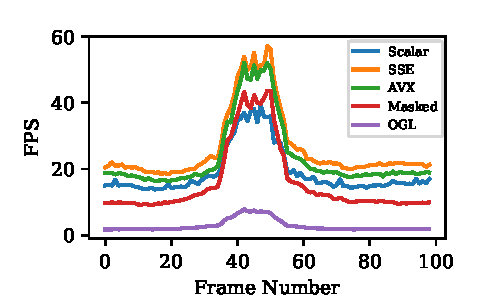
\includegraphics[width=0.5\textwidth]{images/Evaluation_1_Results_FPS.pdf}
		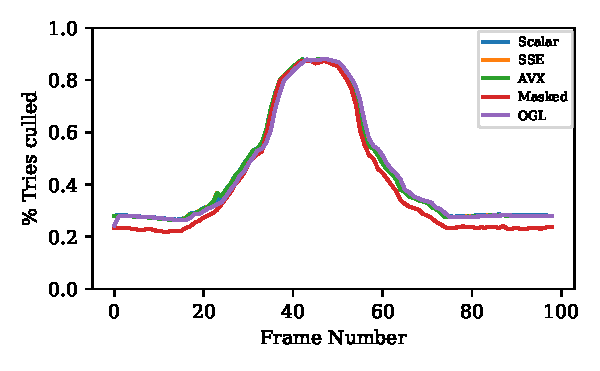
\includegraphics[width=0.5\textwidth]{images/Evaluation_1_Results_Percentage culled.pdf}
		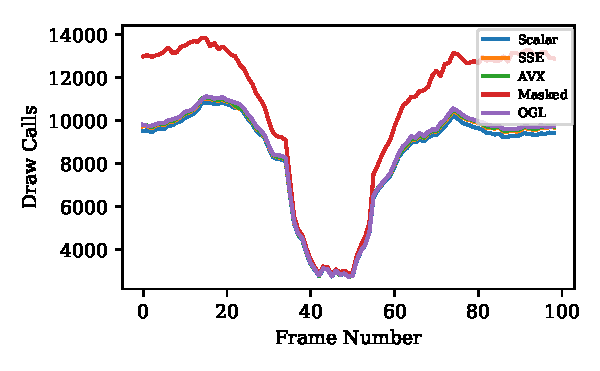
\includegraphics[width=0.5\textwidth]{images/Evaluation_1_Results_Draw Calls.pdf}
		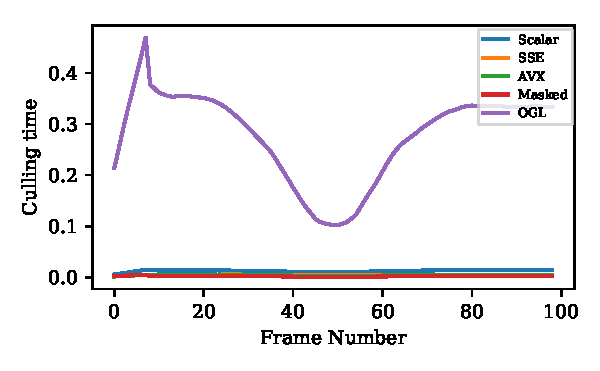
\includegraphics[width=0.5\textwidth]{images/Evaluation_1_Results_Culling time.pdf}
		\caption{Vergleich der 5 verschiedenen Varianten}
		\label{fig:performance_all_5}
	\end{minipage}
\end{figure}

\begin{table}
	\begin{tabular}{| l | r | r | r | r | r |}
		\hline
		                   & Scalar  & SSE     & AVX      & Masked    & OGL      \\ \hline
		FPS                & 24.21   & 29.30   & 26.21    & 22.12     & 3.63     \\ \hline
		Tries culled (\%)  & 43.97   & 43.88   & 43.85    & 40.41     & 43.81    \\ \hline
		Drawcalls          & 8299    & 8442    & 8471     & 10529     & 8514     \\ \hline
		Culling t (ms)     & 11.30   & 4.24    & 3.73     & 1.99      & 292.60   \\ \hline
		Depth Test t (ms)  & 6.90    & 1.59    & 1.72     & 1.45      & 228.38   \\ \hline
		Rasterizer t (ms)  & 4.36    & 2.65    & 2.01     & 2.01      & 64.21    \\ 
		\hline
	\end{tabular}
	\caption{Vergleich der 5 verschiedenen Varianten}
	\label{tbl:performance_all_5}
\end{table}

Unsere Ergebnisse wurden mit dem Intel-Occlusion-Culling-Framework berechnet und verwenden die dortige Testszene einer Burg.
Die Burg hat 115 Occluder mit 48700 Dreiecken und 27025  Occludee Model mit $\approx$ 1923000 Dreiecken.
Unsere Ergebnisse wurden, sofern nicht anders angeben, mit einer Kamerafahrt "uber 100 Frames erstellt.
Der Tiefenbuffer ist standardm"a"sig auf 1920x1080 Pixel gesetzt.
Die Kamera startet mit Blick auf die Burg aus einiger Entfernung und fliegt auf die Burg zu.
An der Burg angekommen dreht sich die Kamera Richtung Boden und entfernt sich anschlie"send wieder von der Burg.
Die Anzahl der Objekte im Sichtfeld ist am Anfang sehr hoch, sinkt in der Mitte der Kamerafahrt ab und steigt am Ende wieder auf den Startwert.
Als Hardware wurde ein Rechner mit einem Intel Core i9-7900X, einer NVIDIA Titan Xp und 64 GB RAM verwendet.

In \autoref{fig:performance_all_5} ist die Leistung der 4 verschiedenen Occlusion Culling Methoden im Intel-Framework im Vergleich zu unserer eigenen Implementierung (OGL) zu sehen.
Die Durchschnittswerte sind in \autoref{tbl:performance_all_5} zu sehen.
Die Anzahl der gecullten Elemente und die Anzahl der Drawcalls ist bei allen Methoden sehr "ahnlich.
Nur das Masked Occlusion Culling cullt $\approx$ 3,5 \% weniger und f"uhrt deswegen mehr Drawcalls aus.

\begin{figure}
	\begin{minipage}{0.5\textwidth}
		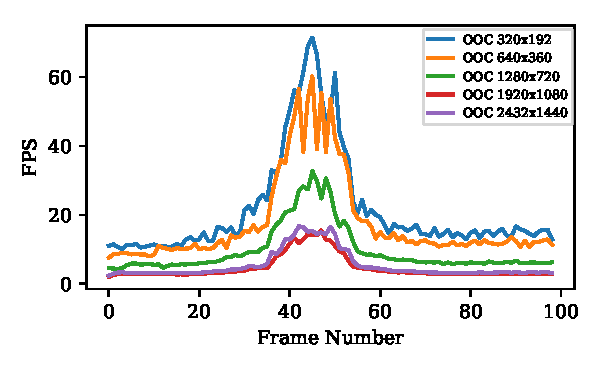
\includegraphics[width=0.5\textwidth]{images/Evaluation_4_Results_FPS.pdf}
		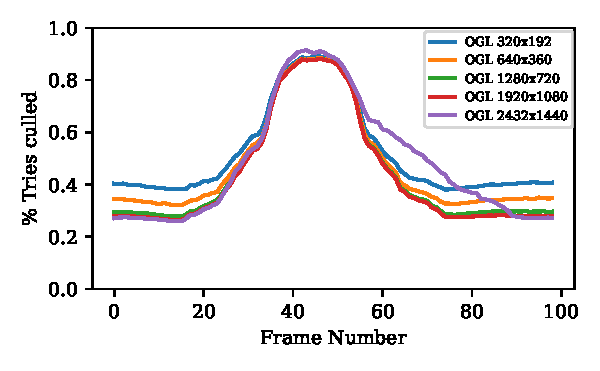
\includegraphics[width=0.5\textwidth]{images/Evaluation_4_Results_Percentage culled.pdf}
		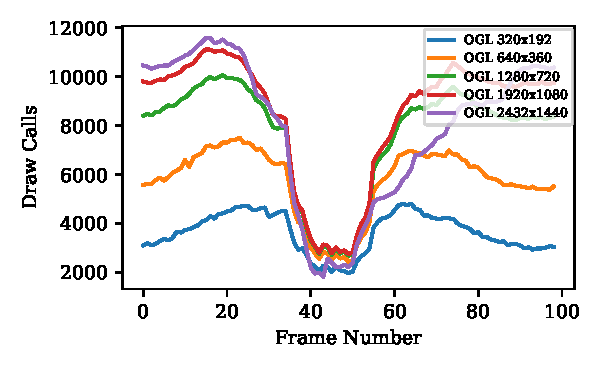
\includegraphics[width=0.5\textwidth]{images/Evaluation_4_Results_Draw Calls.pdf}
		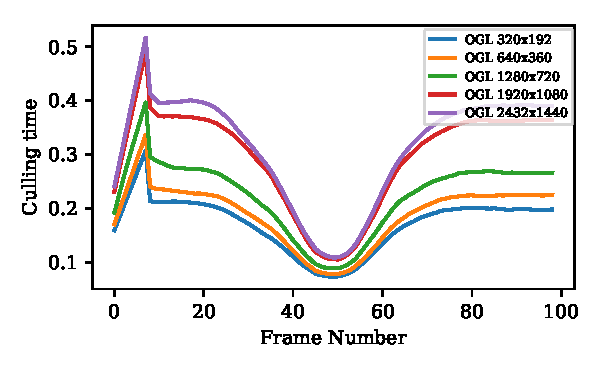
\includegraphics[width=0.5\textwidth]{images/Evaluation_4_Results_Culling time.pdf}
		\caption{OGL mit unterschiedlicher Aufl"osung des Tiefenbuffers}
		\label{fig:different_resolutions}
	\end{minipage}
\end{figure}

\begin{table}
	\begin{tabular}{| l | r | r | r | r | r |}
		\hline
		& 320x192   & 640x360   & 1280x720  & 1920x1080 & 2432x1440 \\ \hline
		FPS                & 6.03      & 5.35      & 4.53      & 3.59      & 3.47      \\ \hline
		Tries culled (\%)  & 51.88     & 47.65     & 44.69     & 43.81     & 48.55     \\ \hline
		Draw Calls         & 3640      & 5759      & 7725      & 8515      & 7920      \\ \hline
		Culling t (ms)     & 171.02    & 188.8     & 223.72    & 295.06    & 312.97    \\ \hline
		Depth Test t (ms)  & 108.86    & 125.27    & 160.27    & 231.08    & 249.05    \\ \hline
		Rasterizer t (ms)  & 62.15     & 63.53     & 63.46     & 63.97     & 63.92     \\
		\hline
	\end{tabular}
	\caption{OGL mit unterschiedlicher Aufl"osung des Tiefenbuffers}
	\label{tbl:different_resolutions}
\end{table}

In \autoref{fig:different_resolutions} wurde unser Programm mit f"unf unterschiedlichen Aufl"osungen des Tiefenbuffers ausgef"uhrt.
Je niedriger die Aufl"osung ist, desto h"ohere Frameraten k"onnen erreicht werden.
Betrachtet man die Werte aus \autoref{tbl:different_resolutions} stellt man fest, dass durch die niedrige Aufl"osung  beim Culling und beim Tiefentest Zeit gespart werden kann.\\


Evaluation 1: alle 5, Kamerafahrt 1\\
Evaluation 2: alle 5, Kamerafahrt 2\\
Evaluation 3: alle 5, DB\_Very\_Large vs DB\_Small\\
Evaluation 4: OGL, alle 5 Aufl"osungen\\
Evaluation 5: OGL, mit und ohne Frustum culling\\
Evaluation 6: alle 5 + OGL ohne Mesa\\
Evaluation 7: OGL + SSE, MT / MT + Frustum Culling / MT + Frustum Culling + Depth Test Culling\\
Evaluation 8: OGL + SSE, Depth Test Tasks 5 / 20 / 100

\begin{figure}
	\begin{minipage}{0.5\textwidth}
		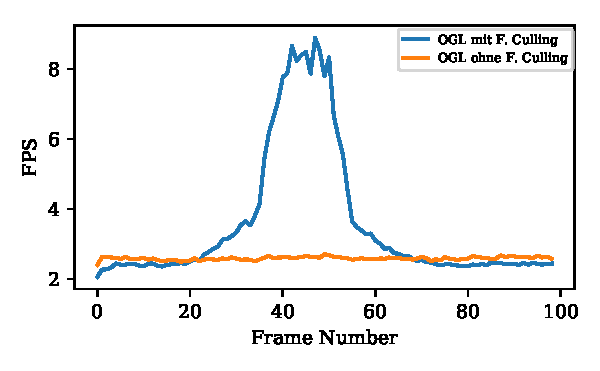
\includegraphics[width=0.5\textwidth]{images/Evaluation_5_Results_FPS.pdf}
		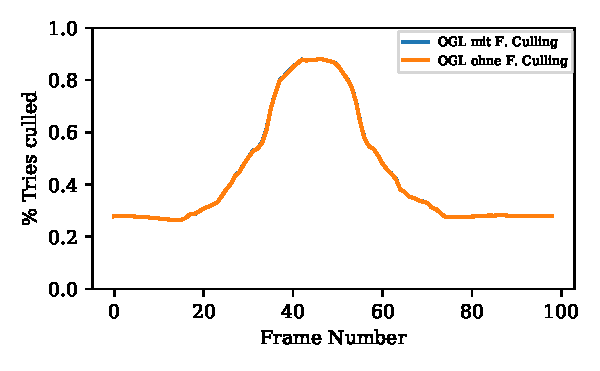
\includegraphics[width=0.5\textwidth]{images/Evaluation_5_Results_Percentage culled.pdf}
		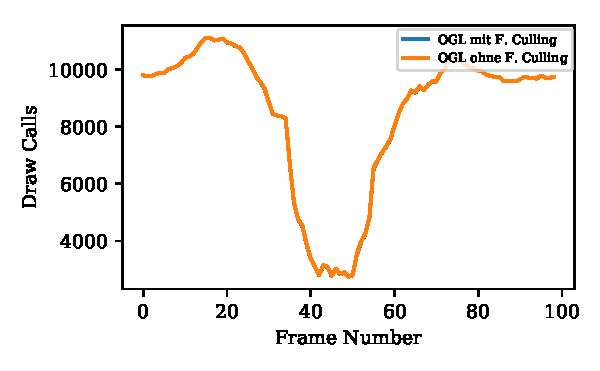
\includegraphics[width=0.5\textwidth]{images/Evaluation_5_Results_Draw Calls.pdf}
		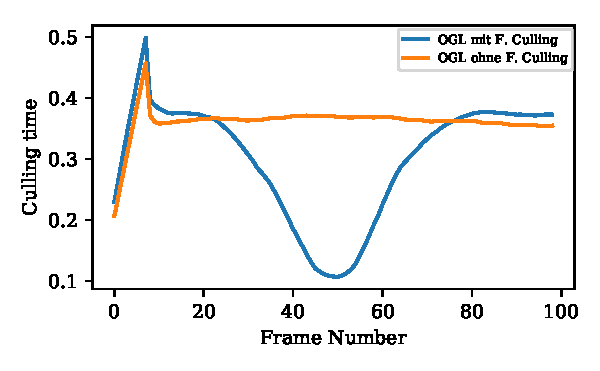
\includegraphics[width=0.5\textwidth]{images/Evaluation_5_Results_Culling time.pdf}
		\caption{OGL mit und ohne Frustum Culling}
		\label{fig:performance_frustum}
	\end{minipage}
\end{figure}

\begin{figure}
	\begin{minipage}{0.5\textwidth}
		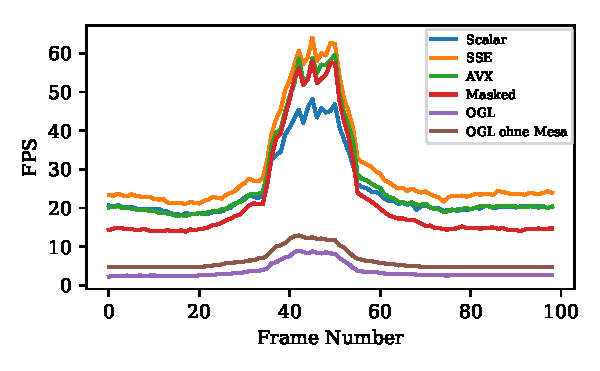
\includegraphics[width=0.5\textwidth]{images/Evaluation_6_Results_FPS.pdf}
		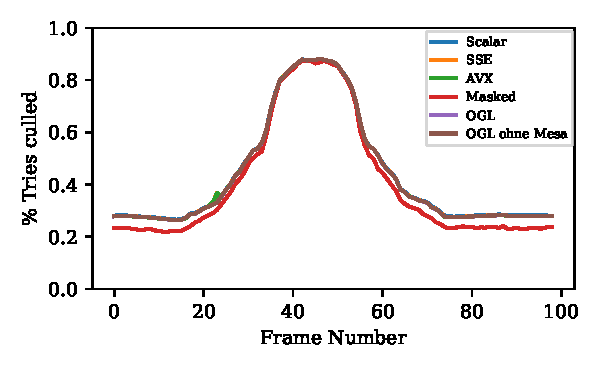
\includegraphics[width=0.5\textwidth]{images/Evaluation_6_Results_Percentage culled.pdf}
		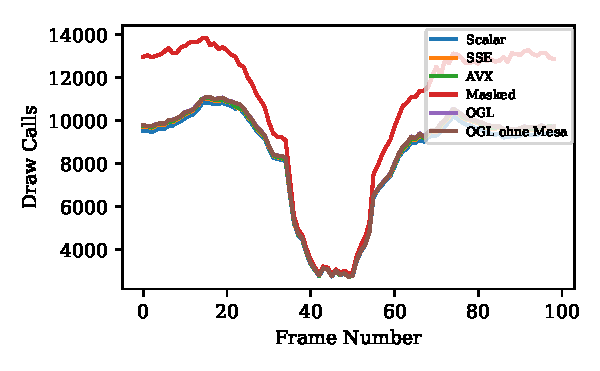
\includegraphics[width=0.5\textwidth]{images/Evaluation_6_Results_Draw Calls.pdf}
		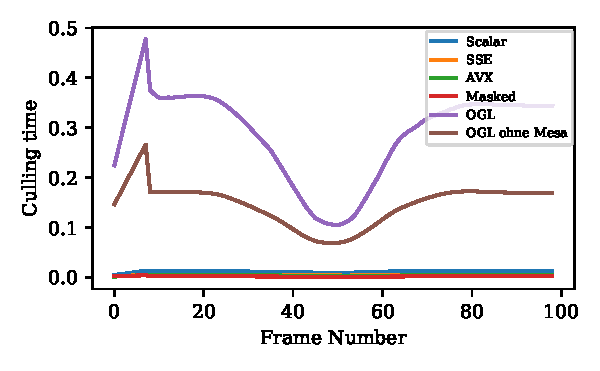
\includegraphics[width=0.5\textwidth]{images/Evaluation_6_Results_Culling time.pdf}
		\caption{Vergleich der 5 verschiedenen Varianten + OGL ohne OSMesa}
		\label{fig:performance_OSMesa}
	\end{minipage}
\end{figure}

\section{Fazit}
Das ist ein Testsatz f"ur das Fazit.

\bibliographystyle{abbrv} 
%% use following if all content of bibtex file should be shown
% \nocite{*}
\bibliography{literatur}
\end{document}
